\subsection{Waiting time} \label{sec:waiting_time}

Waiting time is the amount of time that patients wait in 
the hospital's waiting space before they can receive their service. 
For a given set of parameters there are three different performance measures 
around the mean waiting time that can be calculated. The mean waiting time of
type 1 individuals:

\begin{equation} \label{eq:closed_form_waiting_type_1}
    W^{(1)} = \frac{\sum_{\substack{(u,v) \, \in S_A^{(1)} \\ v \geq C}} 
    \frac{1}{C \mu} \times (v-C+1) \times \pi(u,v)}{\sum_{(u,v) \, 
    \in S_A^{(1)}} \pi(u,v)}
\end{equation}

The mean waiting time of type 2 individuals:

\begin{equation}\label{eq:closed_form_waiting_type_2}
    W^{(2)} = \frac{\sum_{\substack{(u,v) \, \in S_A^{(2)} \\ min(v,T) \geq C}} 
    \frac{1}{C \mu} \times (\min(v+1,T)-C) \times \pi(u,v)}{\sum_{(u,v) \, 
    \in S_A^{(2)}} \pi(u,v)}
\end{equation} 

The overall mean waiting time:

\begin{equation}\label{eq:overall_waiting_time}
    W = \frac{\lambda_1 P_{L'_1}}{\lambda_2 P_{L'_2} + \lambda_1 P_{L'_1}} W^{(1)} 
    + \frac{\lambda_2 P_{L'_2}}{\lambda_2 P_{L'_2} + \lambda_1 P_{L'_1}} W^{(2)}
\end{equation}
 
Here \(S_A^{(1)}\) and \(S_A^{(2)}\) are the set of accepting states for type
1 and type 2 individuals. These are the set of states that the model is able
to accept a specific type of individuals.

\begin{equation}\label{eq:accepting_states_type_1}
    S_A^{(1)} = \{(u, v) \in S \; | \; v < N \}
\end{equation}

\begin{equation}\label{eq:accepting_states_type_2}
    S_A^{(2)}=
    \begin{cases}
        \{(u, v) \in S \; | \; u < M \}, & \textbf{if } T \leq N\\
        \{(u, v) \in S \; | \; v < N \}, & \textbf{otherwise}
    \end{cases}
\end{equation}

Equation \ref{eq:overall_waiting_time} makes use of the proportion of type 1 
and type 2 individuals that are not lost to the system. These probabilities are 
given by \(P_{L'_1}\) and \(P_{L'_2}\) where:

\begin{equation}\label{eq:proportion_of_accepting_individuals}
    P_{L'_1} = \sum_{(u,v) \, \in S_A^{(1)}} \pi(u,v) \hspace{2cm}
    P_{L'_2} = \sum_{(u,v) \, \in S_A^{(2)}} \pi(u,v)
\end{equation}
 
Appendix \ref{sec:appendix_mean_waiting} gives more details on the recursive
formula that equations (\ref{eq:closed_form_waiting_type_1}),
(\ref{eq:closed_form_waiting_type_2}) and (\ref{eq:overall_waiting_time})
originate from. 

Figure \ref{fig:markov_vs_des_waiting_time_comparison_overall} shows a 
comparison between the calculated mean waiting time using Markov chains and the
simulated waiting time using discrete event simulation over a range of values of 
\(\lambda_2\) (details of the discrete event simulation model are given in 
appendix~\ref{sec:appendix_des}).
The figure is used to demonstrate the accuracy of the waiting time formula of
the constructed queueing model as well as the effect of truncating the model.
The simulation was ran 100 times and the recorded mean waiting time at each 
iteration is used to populate the violin plots.
In detail, figure \ref{fig:markov_vs_des_waiting_time_comparison_overall} shows
the calculated mean waiting time using the Markov chain, using a truncated 
simulation and using a simulation with infinite capacity (without the artificial
parameters \(N\) and \(M\)).
Each plot corresponds to different values of \(N\) and \(M\) and is run over 
different values of \(\lambda_2\).
The untruncated simulation values are the same at all three graphs since
the effect of truncation does not apply to it.
The waiting times generated by the truncated simulation match the ones generated 
by the Markov chains model.
Note that this comparison includes both type 1 and type 2 individuals.
A separate comparison of only type 1 and only type 2 individuals can be found 
in appendix~\ref{sec:appendix_additional_figures}.

\begin{figure}[H]
    \centering
    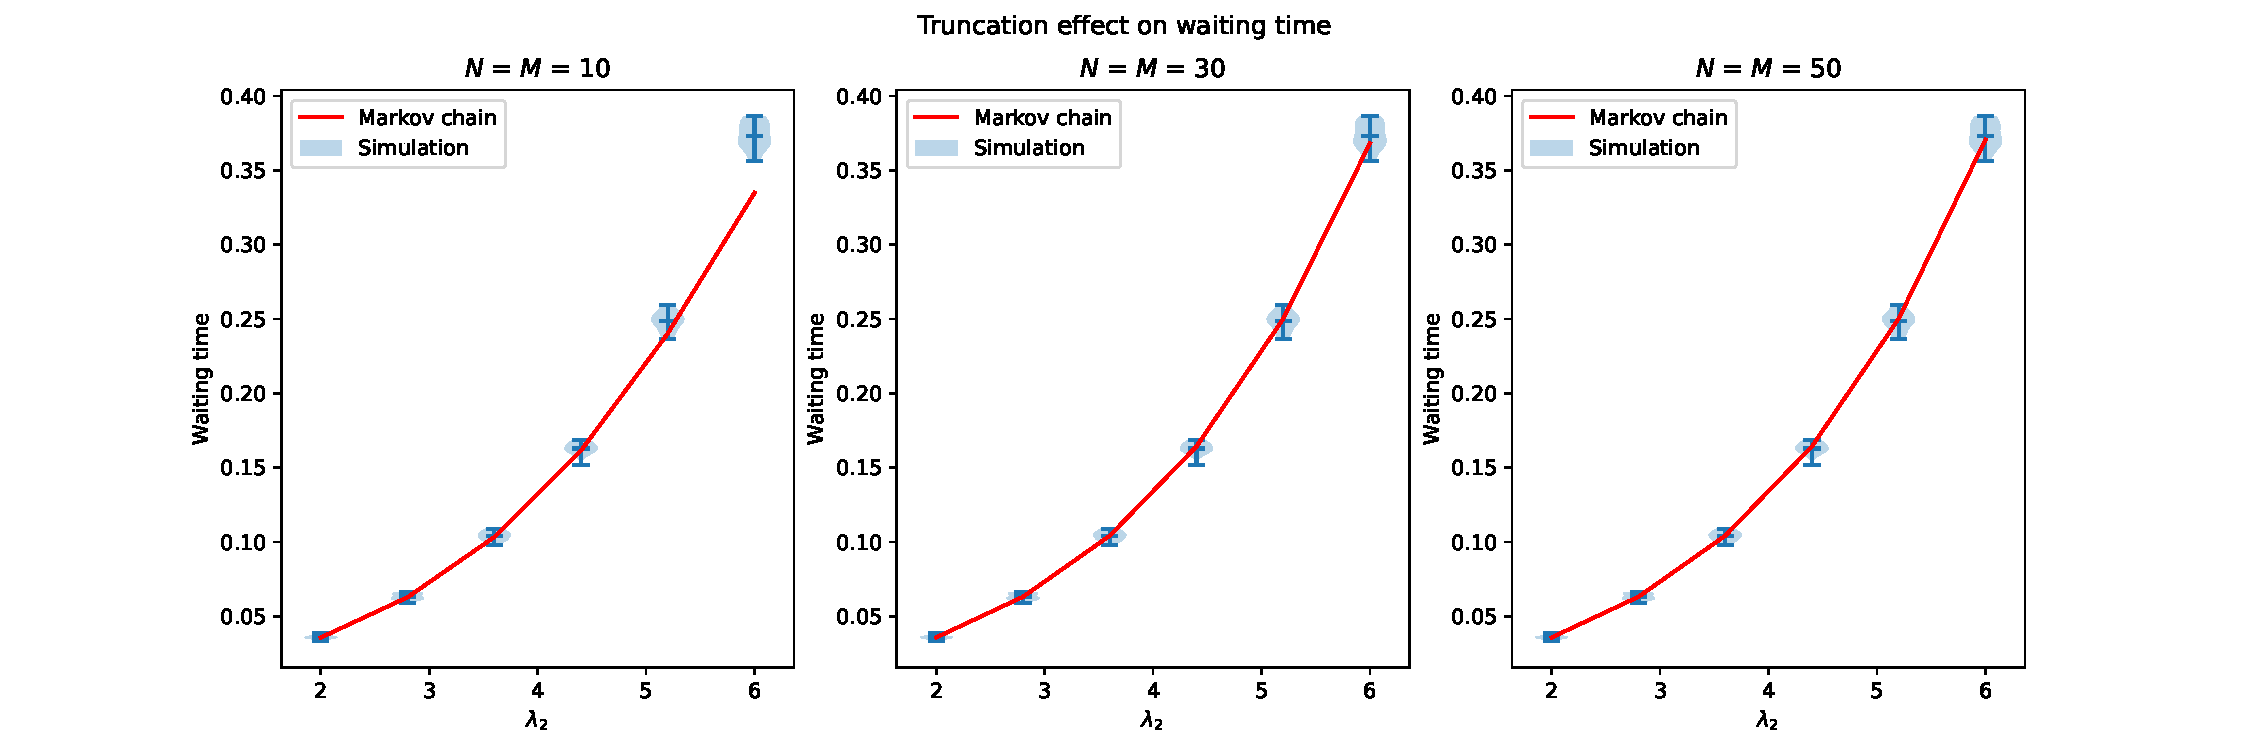
\includegraphics[width=\textwidth]{imgs/truncation_effect/waiting/main.pdf}
    \caption{
        Comparison of mean waiting time between values obtained from the Markov 
        chain formula, values obtained from the truncated simulation and values
        obtained from the untruncated simulation.
    }
    \label{fig:markov_vs_des_waiting_time_comparison_overall}
\end{figure}
